\section{Donald Knuth and the Birth of Computational Complexity Analysis: Measuring the Cost of Logic}

After Backus gave us the compiler—letting humans describe algorithms in a high-level language—the next obvious question arose:

\begin{quote}
\textbf{How expensive is an algorithm?}
\end{quote}

It was no longer enough to ask whether a program \textit{worked}.
You had to ask \textit{how efficiently} it worked.
Could it scale? Could it survive on the primitive computers of the day? Could it beat a naive competitor?

Enter \textbf{Donald Knuth}.

\subsection{The Problem: Algorithms Without Accountability}

In the 1950s and early 1960s, algorithms were often presented like magic tricks:

\begin{itemize}
    \item Here’s a clever method.
    \item Here’s why it gives the correct answer.
    \item Trust me—it’s fast enough.
\end{itemize}

There was little systematic effort to quantify exactly how many steps an algorithm would take, how memory usage would grow, or how performance would scale with larger inputs.

Programs were correct—or incorrect.  
Fast—or slow.  
But \textit{how fast}? \textit{How slow}? Nobody had a consistent way to say.

\subsection{Knuth’s Insight: Count the Operations}

Donald Knuth introduced a radical idea into computer science:  
Algorithms should be treated like mathematical objects—not just proved correct, but \textbf{analyzed}.

In particular:

\begin{itemize}
    \item Measure how many basic operations an algorithm performs as a function of input size \( n \).
    \item Understand how performance grows: linearly, quadratically, logarithmically, or worse.
    \item Classify algorithms not by informal claims, but by asymptotic behavior.
\end{itemize}

Knuth popularized formal tools like:

\begin{itemize}
    \item \textbf{Big-O notation} (\( O(n) \), \( O(n^2) \), \( O(\log n) \)) — bounding the worst-case growth of an algorithm.
    \item \textbf{Amortized analysis} — understanding the average cost over a sequence of operations.
    \item \textbf{Precise counting} — tallying comparisons, swaps, memory accesses, and more.
\end{itemize}

\begin{quote}
It wasn’t enough to have an algorithm that worked.  
You had to know exactly how badly it would betray you at scale.
\end{quote}

\subsection{The Magnum Opus: \textit{The Art of Computer Programming}}

In 1968, Knuth published Volume 1 of what would become one of the most ambitious projects in the history of computing:  
\textbf{\textit{The Art of Computer Programming}}.

This wasn’t just a book—it was a cathedral:

\begin{itemize}
    \item A systematic, rigorous catalog of algorithms, data structures, and complexity analyses.
    \item A treatise that connected programming, mathematics, and engineering in a single intellectual framework.
    \item A declaration that computer science wasn’t just practical—it was deeply theoretical, and deserving of mathematical depth.
\end{itemize}

Knuth’s insistence on analyzing algorithm performance turned "software engineering" into an exact science, where intuition had to be backed by asymptotic proofs.

\subsection{Conclusion: From Algorithms to Asymptotics}

Donald Knuth didn’t just help us build better algorithms.  
He helped us \textbf{understand} them.

Because of Knuth:

\begin{itemize}
    \item Algorithms became objects of formal analysis, not just clever tricks.
    \item Computer science adopted asymptotic thinking as a core tool.
    \item Complexity theory grew from an informal curiosity into a mathematical discipline.
\end{itemize}

\begin{quote}
Before Knuth, algorithms were recipes. After Knuth, algorithms became measurable machinery.
\end{quote}


\begin{figure}[H]
    \centering
    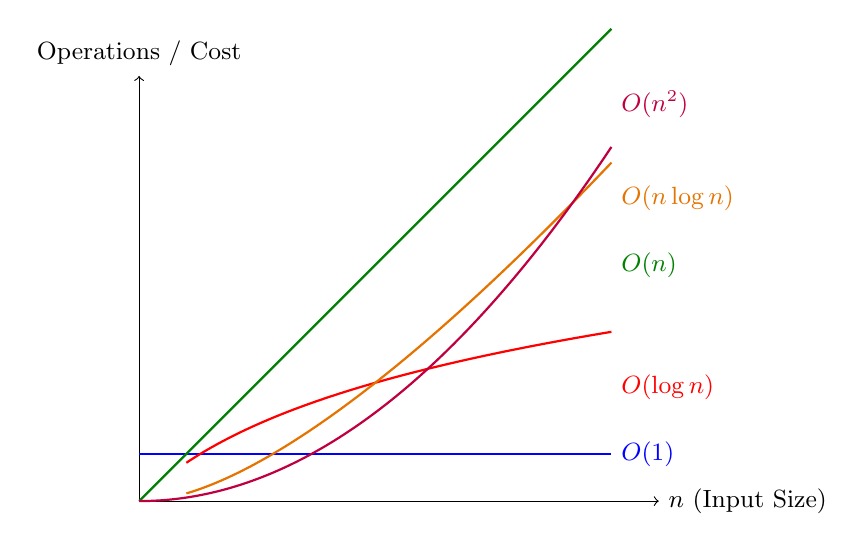
\begin{tikzpicture}[scale=1.2, every node/.style={font=\small}]
      % Axes
      \draw[->] (0,0) -- (5.5,0) node[right] {$n$ (Input Size)};
      \draw[->] (0,0) -- (0,4.5) node[above] {Operations / Cost};
      
      % Functions
      \draw[thick, domain=0:5, samples=100, blue] plot (\x, 0.5);
      \draw[thick, domain=0.5:5, samples=100, red] plot (\x, {ln(\x+1)});
      \draw[thick, domain=0:5, samples=100, green!50!black] plot (\x, \x);
      \draw[thick, domain=0.5:5, samples=100, orange!90!black] plot (\x, {\x*ln(\x+1)/2.5});
      \draw[thick, domain=0:5, samples=100, purple] plot (\x, {0.15*\x*\x});
    
      % Labels
      \node[anchor=west, blue] at (5,0.5) {$O(1)$};
      \node[anchor=west, red] at (5,1.2) {$O(\log n)$};
      \node[anchor=west, green!50!black] at (5,2.5) {$O(n)$};
      \node[anchor=west, orange!90!black] at (5,3.2) {$O(n \log n)$};
      \node[anchor=west, purple] at (5,4.2) {$O(n^2)$};
    
    \end{tikzpicture}
    \caption{Growth Curves of Common Complexity Classes}
    \label{fig:complexity-curves}
\end{figure}
    